\begin{center}
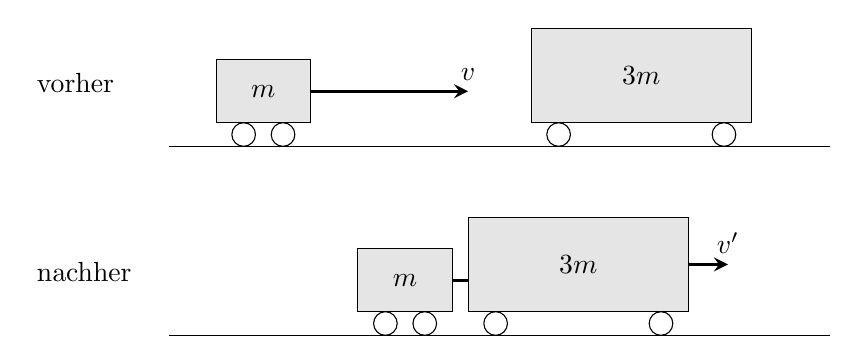
\begin{tikzpicture}[>=stealth]
 \node[anchor=west] at (0,0.8) {vorher};
 \draw (1.8,0) -- (10.2,0);
 \draw[fill=gray!20] (2.4,0.3) rectangle (3.6,1.1);
 \node at (3,0.7) {$m$};
 \draw[fill=white] (2.75,0.15) circle (0.15) (3.25,0.15) circle (0.15);
 \draw[->, very thick] (3.6,0.7) -- (5.6,0.7) node[above] {$v$};
 \draw[fill=gray!20] (6.4,0.3) rectangle (9.2,1.5);
 \node at (7.8,0.9) {$3m$};
 \draw[fill=white] (6.75,0.15) circle (0.15) (8.85,0.15) circle (0.15);
 \node[anchor=west] at (0,-1.6) {nachher};
 \draw (1.8,-2.4) -- (10.2,-2.4);
 \draw[fill=gray!20] (4.2,-2.1) rectangle (5.4,-1.3);
 \node at (4.8,-1.7) {$m$};
 \draw[fill=white] (4.55,-2.25) circle (0.15) (5.05,-2.25) circle (0.15);
 \draw[very thick] (5.4,-1.7) -- (5.6,-1.7);
 \draw[fill=gray!20] (5.6,-2.1) rectangle (8.4,-0.9);
 \node at (7,-1.5) {$3m$};
 \draw[fill=white] (5.95,-2.25) circle (0.15) (8.05,-2.25) circle (0.15);
 \draw[->, very thick] (8.4,-1.5) -- (8.9,-1.5) node[above] {$v'$};
\end{tikzpicture}
\end{center}

Der Gesamtimpuls bleibt erhalten. Nach dem Stoss bewegen sich beide Wagen, zusammen mit der Masse $4m$, mit derselben Geschwindigkeit $v'$:
\begin{align}
 m\,v &= \left(m+3m\right)v' = 4m\,v'
\end{align}
Also ist
\begin{align}
 v' &= \vGeF = \frac{\vWa}{4} = \vGe \approx \result{\vGeP{0}{2}}
\end{align}
